\section{Additional CIFAR models, training controls, and semantic checks}
\label{sec:supp_additional_cifar}

These completed studies test which conclusions survive a stronger pretrained
model, matched training controls, and a second classifier representation.
They complement the five-panel DDPM confirmation in the main paper; their KID, coverage, and regional-mass results are
\emph{descriptive development measurements}, with one noise panel per arm.
All declared arms are reported below. The additional studies reuse the
10,000-image CIFAR test reference. Only completed study arms contribute to these tables.

\subsection{Cost-matched solver comparisons on EDM}
We use the official unconditional CIFAR-10 VP checkpoint from
EDM~\cite{karras2022edm}, independently pretrained from the public DDPM.
The official implementation is pinned to commit
\texttt{008a4e5316c8e3bfe61a\allowbreak{}62f874bddba254295afb}; checkpoint and source
hashes are retained with the protocol. Sampling uses the power-law noise
grid with $\rho=7$, $\sigma_{\min}=0.002$, $\sigma_{\max}=80$, and
zero stochastic churn. Integration is in FP64 and the network is in FP32,
as in the official implementation. The official conversion to uint8 is
$\operatorname{clip}(127.5x+128,0,255)$, followed by integer conversion.

Euler requires one denoiser call per step. Heun requires two except at the
final step, so $K$ Heun steps require $2K-1$ calls. The complete comparison
pairs Euler at 3/7/15/35 steps with Heun at 2/4/8/18 steps.
This matches denoiser calls while allowing their integration grids to differ;
it does not isolate formal order on an identical grid. All eight arms use
2,048 paired per-image seeds beginning at 97,000,000, batch size 64, and
no result-dependent choice of seeds. Instrumented call counts and a
same-input comparison against the official Heun sampler verify the adapter:
uint8 outputs agree exactly, and floating outputs differ by at most
$10^{-10}$ under the declared check. Total generation is 16,384 images and
245,760 forward-image calls.

Table~\ref{tab:additional_edm} reports all outcomes.
At 15 calls, Heun lowers KID by 71.4\%, but its coverage and precision
are lower. At 35 calls, Heun lowers KID by 83.5\% with essentially unchanged
coverage, while its accepted-class mass error is higher. At three and
seven calls the KID ordering reverses. The joint pattern is informative:
higher integration order helps only when enough integration intervals
remain, and a better distributional quality metric need not improve every
coverage or regional statistic. High DINO precision on the three-call
Euler output is particularly misleading when considered alone: its
classifier acceptance is 1.37\%, recall is 0.026, and coverage is 0.111.
Figure~\ref{fig:edm_fixed_examples} shows the first two paired noise indices
for every arm, without ranking or replacement.

% BEGIN AUTO EDM
\begin{table*}[t]
\centering\small
\setlength{\tabcolsep}{4pt}
\caption{Complete EDM comparison. Each arm uses the same 2,048 noise seeds. Calls count denoiser evaluations; Heun uses $2K-1$ calls for $K$ steps. KID is multiplied by $10^3$; P/C/R/D are fixed-real DINO precision, coverage, recall, and density ($k=5$). MAD is the mean absolute error of ten unconditional accepted-region masses; Acc. is classifier acceptance. These are descriptive development points. Seconds are observed generation time, excluding feature extraction, on a shared H200; call counts are the controlled cost.}
\label{tab:additional_edm}
\begin{tabular}{lrrrrrrrrr}
\toprule
Sampler & Calls & KID$\downarrow$ & P & C & R & D & MAD$\downarrow$ & Acc. & Sec. \\
\midrule
Euler 3 & 3 & 202.607 & 0.868 & 0.111 & 0.026 & 3.229 & 0.0894 & 0.0137 & 14.9 \\
Heun 2 & 3 & 649.138 & 0.000 & 0.000 & 0.000 & 0.000 & 0.0907 & 0.0000 & 14.6 \\
Euler 7 & 7 & 36.549 & 0.881 & 0.341 & 0.409 & 2.320 & 0.0376 & 0.6284 & 34.1 \\
Heun 4 & 7 & 98.298 & 0.906 & 0.191 & 0.135 & 5.023 & 0.0705 & 0.3379 & 33.9 \\
Euler 15 & 15 & 8.758 & 0.856 & 0.477 & 0.638 & 1.423 & 0.0142 & 0.8418 & 73.0 \\
Heun 8 & 15 & 2.504 & 0.787 & 0.417 & 0.692 & 1.006 & 0.0118 & 0.8311 & 72.6 \\
Euler 35 & 35 & 2.500 & 0.821 & 0.501 & 0.716 & 1.136 & 0.0070 & 0.8862 & 170.3 \\
Heun 18 & 35 & 0.413 & 0.799 & 0.501 & 0.741 & 1.053 & 0.0103 & 0.8872 & 169.2 \\
\bottomrule
\end{tabular}
\end{table*}
% END AUTO EDM

\begin{figure*}[t]
\centering
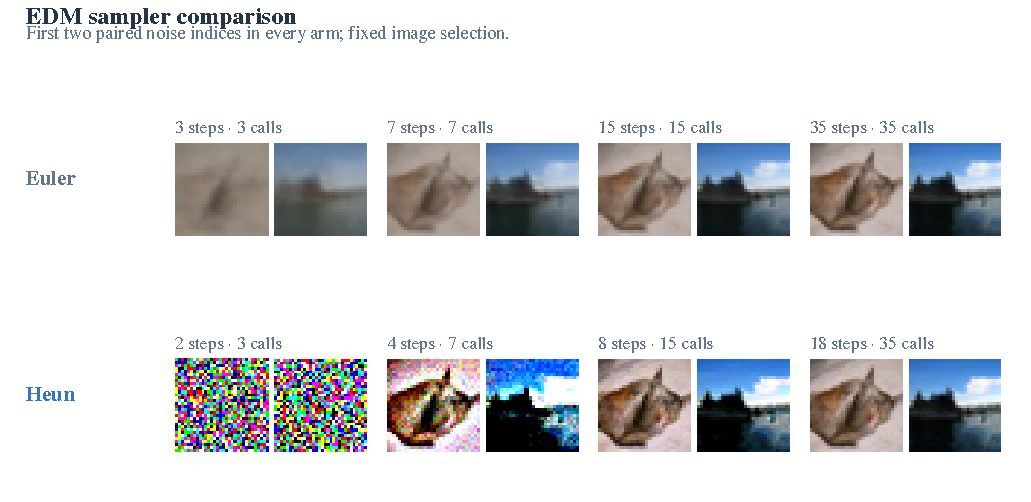
\includegraphics[width=\textwidth]{../figures/edm_quality_examples.pdf}
\caption{All eight EDM arms, using the first two fixed paired noise indices.
They are the first two indices of the prespecified first-12 example set,
with no ranking or replacement. Matching
calls changes the number of Euler versus Heun integration intervals; the
three- and seven-call failures are retained alongside the higher-budget
outputs. Quantitative conclusions use all 2,048 images per arm.}
\label{fig:edm_fixed_examples}
\end{figure*}

\paragraph{Image-frequency cross-check.}
An additional completed check measures the mean squared magnitude of the
unnormalized grayscale $32\times32$ Fourier transform outside centered
radius eight. The range is fixed from 10,000 real training images:
the 1--99\% quantile band is $[2.53593,41.11845]$, and the declared
5--95\% sensitivity band is $[4.37764,30.74381]$ (linear quantiles).
The check was motivated by visible artifacts in development images;
it is an artifact proxy, rather than a universal visual-quality definition.
It can reject legitimate unusually smooth or textured images.
The complete record covers all 58 available cached arms; the EDM arms
and relevant DDPM reference/initializer controls are shown in
Table~\ref{tab:additional_frequency}. The archived frequency display retains marginal precision and primary-band
rates with pointwise 95\% Clopper--Pearson intervals, conditional on the fixed
band. They are separate from simultaneous fidelity certification.

At seven calls, Heun's DINO precision is 0.906 but its frequency-range
rate is only 0.247. At 35 calls, Heun's frequency-range rate rises to
0.978 despite lower DINO precision. The DDPM covariance initializer also
improves the frequency-range rate from 0.0072 to 0.2470, while leaving a
substantial gap to DDIM200's 0.9720. Thus its replicated KID improvement
and coverage gain repair part of the low-budget failure; they do not
establish complete real-data fidelity. The narrower-band results and
conjunction with the fixed DINO precision event remain visible below.

% BEGIN AUTO ARTIFACT
\begin{table*}[t]
\centering\small
\setlength{\tabcolsep}{4pt}
\caption{Frequency-range cross-check: all eight EDM arms and DDPM initializer/reference controls. P is the same fixed-real DINO precision event used in each completed record. F$_{98}$ and F$_{90}$ are the fractions within the 1--99\% and 5--95\% real-training frequency ranges; P$\cap$F is their measured conjunction, not a product of marginal rates. Rows are descriptive, with no simultaneous quality certification.}
\label{tab:additional_frequency}
\begin{tabular}{lrrrrrr}
\toprule
Arm & $n$ & P & F$_{98}$ & P$\cap$F$_{98}$ & F$_{90}$ & P$\cap$F$_{90}$ \\
\midrule
Euler 3 & 2,048 & 0.8682 & 0.0137 & 0.0132 & 0.0010 & 0.0010 \\
Heun 2 & 2,048 & 0.0000 & 0.0000 & 0.0000 & 0.0000 & 0.0000 \\
Euler 7 & 2,048 & 0.8813 & 0.4492 & 0.3950 & 0.1860 & 0.1621 \\
Heun 4 & 2,048 & 0.9058 & 0.2466 & 0.2212 & 0.0776 & 0.0718 \\
Euler 15 & 2,048 & 0.8560 & 0.8853 & 0.7563 & 0.6772 & 0.5854 \\
Heun 8 & 2,048 & 0.7871 & 0.9058 & 0.7163 & 0.7427 & 0.5845 \\
Euler 35 & 2,048 & 0.8213 & 0.9629 & 0.7905 & 0.8730 & 0.7197 \\
Heun 18 & 2,048 & 0.7988 & 0.9780 & 0.7827 & 0.8940 & 0.7197 \\
DDPM leading2 & 10,000 & 0.9410 & 0.0072 & 0.0067 & 0.0005 & 0.0005 \\
DDPM initial covariance2 & 10,000 & 0.9544 & 0.2470 & 0.2348 & 0.1003 & 0.0947 \\
DDPM DDIM200 & 2,000 & 0.7890 & 0.9720 & 0.7650 & 0.9000 & 0.7065 \\
\bottomrule
\end{tabular}
\end{table*}
% END AUTO ARTIFACT

\subsection{Matched natural-image training controls}
\paragraph{Training and pairing.}
All three adapted states start from the same public
\texttt{google/ddpm-cifar10-32} checkpoint, pinned to revision
\texttt{267b167dc01f0e4e6192\allowbreak{}3ea244e8b988f84deb80}.
They receive 3,000 updates with one shared adaptation seed, 85,001,
batch size 128, learning rate $2\times10^{-5}$, dropout 0.1, and a new
Adam state because the public checkpoint contains no optimizer state.
Adam uses $(\beta_1,\beta_2)=(0.9,0.999)$, $\epsilon=10^{-8}$, and
zero weight decay. We clip the gradient norm to one and maintain an EMA
with decay 0.999, initialized from the public weights.
The objective is epsilon-prediction MSE with a uniformly sampled timestep:
$x_t=\sqrt{\bar\alpha_t}x_0+\sqrt{1-\bar\alpha_t}\epsilon$.
There are 1,000 training noise levels with linear betas from $10^{-4}$ to
0.02. Images are mapped to $[-1,1]$ and flipped horizontally with
probability 0.5. Forward computation uses BF16; model masters, loss,
Adam state, and EMA use FP32, with TF32 disabled and deterministic
algorithms enabled.

The controls change only the distribution used to draw labeled training
examples. \emph{Uniform} samples all ten classes equally.
\emph{Cat $3\times$} repeats each cat example three times, so cats have
25\% of the resulting 60,000-example mixture.
\emph{Ratio} uses all ten classifier-event residuals from an earlier,
disjoint 2,000-image public DPM++25 pilot. Let $p_j$ and $q_j$ denote the
unconditional accepted-region frequencies in the real reference and that
pilot, and let $p_R,q_R$ be rejection frequencies. The heuristic sets
weights $w_j$ by clipping the accepted-only frequency ratio to $[0.5,2]$
and normalizes them over the ten classes indexed by $k$:
\begin{equation}
\begin{aligned}
 w_j&=\operatorname{clip}\!\left(
 \frac{p_j/(1-p_R)}{q_j/(1-q_R)},\;0.5,\;2\right),\\
 \Pr(\text{training class}=j)&=\frac{w_j}{\sum_k w_k}.
\end{aligned}
\label{eq:supp_class_weighting}
\end{equation}
The class probabilities in label order, rounded here to four decimals, are
0.1239, 0.0835, 0.1289, 0.0670, 0.1120, 0.1019, 0.0528, 0.0958,
0.1407, and 0.0934. Exact values are frozen in the training protocol.
The ratio is an intervention hypothesis, not an inverse model of how
training frequencies determine generated frequencies.

Uniform and Ratio consume the same uniform random draws through their
inverse sampling CDFs. A saved check verifies matching RNG consumption
against the existing cat branch, including subsequent flips, noise,
timesteps, and dropout. Checkpoints every 500 updates retain model, EMA,
optimizer, RNG states, and hashes; full per-update histories are preserved.
A five-update interrupted/resumed segment reproduces model, EMA, Adam,
RNG state, and losses exactly. This pairing controls optimization noise
within the study; one adaptation seed does not quantify across-training
variability, and all branches share one pretrained base.

\paragraph{Complete evaluation.}
The unmodified public state and all three adapted states are evaluated
with DDIM25, DDIM50, and DPM++25. A separately declared extension evaluates
DPM++8 and UniPC8 on the same four states. All use trailing timesteps,
2,000 paired fresh seeds 98,000,000--98,001,999, FP32 sampling, batch 128,
and the same frozen classifiers and feature extractors. Generation totals
40,000 images and 928,000 forward-image calls; the two newly trained
controls add 6,000 optimizer updates. Table~\ref{tab:additional_training}
retains all 20 arms. The main text's public DPM++25 control is regenerated
on this fresh panel; the older pilot is used only to define the Ratio
weights and the separate reference-sensitivity check.

The regional error is
$\operatorname{MAD}_{10}=\frac{1}{10}\sum_{j=0}^9|q_j-p_j|$,
with all samples, including rejected images, in each denominator.
Thus a high rejection rate cannot disappear through renormalization.
KID is the unbiased cubic-kernel MMD in Inception features against the
fixed 10,000-image real reference. DINO precision uses membership in the
union of those real images' fifth-neighbor balls; coverage is the fraction
of real balls reached by any generated point. Recall uses generated
fifth-neighbor balls, and density averages the number of real balls
containing each generated point, divided by five.
These are the exact fixed-real events used in the reported quality gates;
values from a differently subsampled PRDC reference are not substituted.

Table~\ref{tab:additional_training_contrasts} preserves every declared
same-sampler comparison. For classifier acceptance and fixed-real DINO
precision, the paired-Bernoulli interval in the methods supplement bounds
the candidate-minus-reference probability difference using four
Clopper--Pearson tails per comparison. We use $\alpha=0.05$, a
five-percentage-point noninferiority margin, and families of 36 and 24
binary comparisons for the long-step and eight-call studies, respectively.
All statements condition on the frozen trained checkpoints, classifiers,
and fixed real geometry. They do not quantify uncertainty over training
seeds. A joint pass requires both event lower bounds to exceed $-0.05$;
otherwise the result can remain inconclusive.

Uniform continuation improves KID and mass error over the public state
under every sampler. The Ratio intervention has worse KID under all five
samplers and worse mass error under the three long-step probes than
Uniform; at eight calls it slightly improves mass error while losing KID
and coverage. Cat oversampling also has worse KID and mass error than
Uniform, and its quality noninferiority relative to Uniform remains
inconclusive under every sampler. These controls show why an observed
class-region residual alone is insufficient to prescribe class reweighting.

% BEGIN AUTO TRAINING
\begin{table*}[t]
\centering\small
\setlength{\tabcolsep}{4pt}
\caption{Complete natural-image training-control study: four states and five samplers, with 2,000 paired fresh noise seeds per arm. Uniform, Ratio, and Cat $3\times$ each receive 3,000 updates from the same public base and one adaptation seed. All point estimates condition on those trained states and the reused real reference; they are not independent-training-seed estimates. P/C/R/D and Acc. have the definitions of Table~\ref{tab:additional_edm}; Cat err. is the absolute error of the unconditional accepted cat-region mass.}
\label{tab:additional_training}
\begin{tabular}{llrrrrrrrr}
\toprule
Sampler & Training & KID$\times10^3\downarrow$ & P & C & R & D & MAD$\downarrow$ & Cat err.$\downarrow$ & Acc. \\
\midrule
DDIM25 & Public & 18.253 & 0.780 & 0.315 & 0.543 & 1.286 & 0.0307 & 0.0218 & 0.7210 \\
DDIM25 & Uniform & 13.307 & 0.791 & 0.350 & 0.578 & 1.136 & 0.0165 & 0.0043 & 0.7515 \\
DDIM25 & Ratio & 13.617 & 0.785 & 0.344 & 0.589 & 1.123 & 0.0178 & 0.0122 & 0.7540 \\
DDIM25 & Cat $3\times$ & 16.382 & 0.795 & 0.347 & 0.585 & 1.351 & 0.0260 & 0.0458 & 0.7395 \\
\midrule
DDIM50 & Public & 13.493 & 0.784 & 0.328 & 0.585 & 1.286 & 0.0248 & 0.0048 & 0.7470 \\
DDIM50 & Uniform & 9.589 & 0.787 & 0.356 & 0.627 & 1.128 & 0.0143 & 0.0047 & 0.7645 \\
DDIM50 & Ratio & 10.051 & 0.784 & 0.349 & 0.626 & 1.090 & 0.0170 & 0.0217 & 0.7770 \\
DDIM50 & Cat $3\times$ & 12.228 & 0.793 & 0.347 & 0.622 & 1.287 & 0.0233 & 0.0343 & 0.7430 \\
\midrule
DPM++25 & Public & 14.786 & 0.752 & 0.308 & 0.600 & 0.996 & 0.0247 & 0.0018 & 0.7375 \\
DPM++25 & Uniform & 10.096 & 0.766 & 0.338 & 0.637 & 0.949 & 0.0148 & 0.0092 & 0.7595 \\
DPM++25 & Ratio & 10.899 & 0.757 & 0.334 & 0.639 & 0.912 & 0.0176 & 0.0212 & 0.7735 \\
DPM++25 & Cat $3\times$ & 12.477 & 0.763 & 0.336 & 0.626 & 1.041 & 0.0242 & 0.0353 & 0.7360 \\
\midrule
DPM++8 & Public & 26.943 & 0.794 & 0.306 & 0.437 & 1.516 & 0.0369 & 0.0558 & 0.6500 \\
DPM++8 & Uniform & 21.767 & 0.805 & 0.336 & 0.490 & 1.281 & 0.0255 & 0.0243 & 0.7010 \\
DPM++8 & Ratio & 22.333 & 0.798 & 0.333 & 0.491 & 1.259 & 0.0242 & 0.0083 & 0.7045 \\
DPM++8 & Cat $3\times$ & 25.118 & 0.799 & 0.328 & 0.495 & 1.435 & 0.0378 & 0.0743 & 0.6785 \\
\midrule
UniPC8 & Public & 25.240 & 0.792 & 0.303 & 0.445 & 1.333 & 0.0359 & 0.0553 & 0.6630 \\
UniPC8 & Uniform & 19.527 & 0.786 & 0.340 & 0.507 & 1.176 & 0.0239 & 0.0263 & 0.7210 \\
UniPC8 & Ratio & 20.391 & 0.780 & 0.334 & 0.505 & 1.142 & 0.0227 & 0.0048 & 0.7135 \\
UniPC8 & Cat $3\times$ & 22.988 & 0.796 & 0.334 & 0.505 & 1.322 & 0.0347 & 0.0673 & 0.6955 \\
\bottomrule
\end{tabular}
\end{table*}
% END AUTO TRAINING

% BEGIN AUTO CONTRASTS
\begin{table*}[t]
\centering\small
\setlength{\tabcolsep}{4pt}
\caption{All 30 declared same-sampler training contrasts. Negative KID and MAD differences favor the first state. Intervals bound the candidate-minus-reference acceptance (Acc.) and fixed-real DINO precision (P) differences. The exact paired-Bernoulli construction controls a 36-event family for the three long-step samplers and a separate 24-event family for the two eight-call samplers; the two families are not jointly a single 95\% statement. Pass requires both lower bounds to exceed $-0.05$. Inconclusive is not a demonstrated quality loss; passing permits losses within the stated margin. Decisions use unrounded bounds; KID/MAD differences are descriptive.}
\label{tab:additional_training_contrasts}
\begin{tabular}{llrrlll}
\toprule
Sampler & Contrast & $\Delta$KID$\times10^3$ & $\Delta$MAD & $\Delta$Acc. interval & $\Delta$P interval & Joint NI \\
\midrule
DDIM25 & Uniform $-$ Public & -4.946 & -0.0143 & [-0.0110, +0.0788] & [-0.0298, +0.0545] & Pass \\
DDIM25 & Ratio $-$ Public & -4.636 & -0.0129 & [-0.0090, +0.0821] & [-0.0382, +0.0494] & Pass \\
DDIM25 & Cat $3\times$ $-$ Public & -1.871 & -0.0048 & [-0.0225, +0.0638] & [-0.0251, +0.0588] & Pass \\
DDIM25 & Ratio $-$ Uniform & +0.310 & +0.0014 & [-0.0330, +0.0388] & [-0.0422, +0.0283] & Pass \\
DDIM25 & Cat $3\times$ $-$ Uniform & +3.075 & +0.0095 & [-0.0502, +0.0226] & [-0.0302, +0.0395] & Inconcl. \\
DDIM25 & Ratio $-$ Cat $3\times$ & -2.765 & -0.0082 & [-0.0237, +0.0565] & [-0.0494, +0.0265] & Pass \\
DDIM50 & Uniform $-$ Public & -3.904 & -0.0105 & [-0.0236, +0.0627] & [-0.0389, +0.0445] & Pass \\
DDIM50 & Ratio $-$ Public & -3.442 & -0.0077 & [-0.0110, +0.0778] & [-0.0439, +0.0428] & Pass \\
DDIM50 & Cat $3\times$ $-$ Public & -1.265 & -0.0014 & [-0.0481, +0.0391] & [-0.0302, +0.0506] & Pass \\
DDIM50 & Ratio $-$ Uniform & +0.463 & +0.0028 & [-0.0192, +0.0484] & [-0.0383, +0.0313] & Pass \\
DDIM50 & Cat $3\times$ $-$ Uniform & +2.640 & +0.0090 & [-0.0603, +0.0106] & [-0.0270, +0.0421] & Inconcl. \\
DDIM50 & Ratio $-$ Cat $3\times$ & -2.177 & -0.0063 & [+0.0002, +0.0771] & [-0.0484, +0.0267] & Pass \\
DPM++25 & Uniform $-$ Public & -4.690 & -0.0099 & [-0.0199, +0.0689] & [-0.0286, +0.0598] & Pass \\
DPM++25 & Ratio $-$ Public & -3.886 & -0.0071 & [-0.0053, +0.0852] & [-0.0398, +0.0498] & Pass \\
DPM++25 & Cat $3\times$ $-$ Public & -2.309 & -0.0005 & [-0.0461, +0.0427] & [-0.0321, +0.0555] & Pass \\
DPM++25 & Ratio $-$ Uniform & +0.803 & +0.0028 & [-0.0179, +0.0505] & [-0.0475, +0.0256] & Pass \\
DPM++25 & Cat $3\times$ $-$ Uniform & +2.381 & +0.0094 & [-0.0634, +0.0093] & [-0.0413, +0.0333] & Inconcl. \\
DPM++25 & Ratio $-$ Cat $3\times$ & -1.577 & -0.0066 & [+0.0030, +0.0812] & [-0.0468, +0.0332] & Pass \\
DPM++8 & Uniform $-$ Public & -5.176 & -0.0114 & [+0.0099, +0.1001] & [-0.0273, +0.0520] & Pass \\
DPM++8 & Ratio $-$ Public & -4.610 & -0.0127 & [+0.0110, +0.1058] & [-0.0379, +0.0457] & Pass \\
DPM++8 & Cat $3\times$ $-$ Public & -1.825 & +0.0008 & [-0.0120, +0.0750] & [-0.0341, +0.0453] & Pass \\
DPM++8 & Ratio $-$ Uniform & +0.566 & -0.0013 & [-0.0306, +0.0387] & [-0.0419, +0.0245] & Pass \\
DPM++8 & Cat $3\times$ $-$ Uniform & +3.351 & +0.0123 & [-0.0617, +0.0103] & [-0.0393, +0.0253] & Inconcl. \\
DPM++8 & Ratio $-$ Cat $3\times$ & -2.784 & -0.0135 & [-0.0099, +0.0684] & [-0.0377, +0.0342] & Pass \\
UniPC8 & Uniform $-$ Public & -5.713 & -0.0119 & [+0.0161, +0.1077] & [-0.0483, +0.0338] & Pass \\
UniPC8 & Ratio $-$ Public & -4.849 & -0.0131 & [+0.0082, +0.1007] & [-0.0559, +0.0281] & Inconcl. \\
UniPC8 & Cat $3\times$ $-$ Public & -2.252 & -0.0012 & [-0.0079, +0.0797] & [-0.0356, +0.0446] & Pass \\
UniPC8 & Ratio $-$ Uniform & +0.864 & -0.0012 & [-0.0433, +0.0261] & [-0.0401, +0.0262] & Pass \\
UniPC8 & Cat $3\times$ $-$ Uniform & +3.461 & +0.0107 & [-0.0641, +0.0056] & [-0.0211, +0.0455] & Inconcl. \\
UniPC8 & Ratio $-$ Cat $3\times$ & -2.597 & -0.0119 & [-0.0189, +0.0595] & [-0.0549, +0.0172] & Inconcl. \\
\bottomrule
\end{tabular}
\end{table*}
% END AUTO CONTRASTS

\subsection{Calibrated classifier regions and reference robustness}
\paragraph{Two-classifier consensus.}
Two CIFAR-stem ResNet-18 classifiers are trained from scratch with seeds
84,001 and 84,002. A single unstratified permutation with seed 84,000
splits the 50,000 training images into 45,000 fitting, 2,500 temperature,
and 2,500 acceptance-calibration images. Both use the fixed final
checkpoint at epoch 200. Training uses batch 256, SGD with learning rate
0.1, momentum 0.9, Nesterov updates, weight decay $5\times10^{-4}$,
five warmup epochs followed by cosine decay, reflect-padding by four
pixels, random $32\times32$ cropping, and horizontal flips.
There is no label smoothing or validation-based checkpoint selection.

Separate temperature fits minimize held-out NLL, giving temperatures
1.29126 and 1.27755. An image is accepted only when both classifiers
predict the same class and both calibrated maximum probabilities exceed
a common threshold. Before training, we declare the 14 thresholds
$\{.5,.6,.7,.75,.8,.85,.9,.92,.94,.96,.97,.98,.99,.995\}$.
The lowest eligible threshold must accept at least 500 calibration images
and have a one-sided Clopper--Pearson selective-error upper bound at most
0.02, using tail probability $0.05/14$ to account for threshold selection.
The selected threshold is 0.8: 24 errors among 2,310 accepted calibration
images yield an upper bound of 0.01748. Only then is the official test set
used for reporting. Individual test accuracies are 95.32\% and 95.30\%;
consensus accepts 9,075/10,000 images with 98.7548\% accuracy among them.
Class-region masses are compared with these measured real accepted-region
masses, rather than the nominal 0.1 label proportions.

The guarantee concerns real validation inputs under the sampling
assumption. It does not establish generated-image semantic correctness.
Accordingly, we call these \emph{accepted classifier regions}, retain the
reject event, and inspect unranked examples. No human annotation or
true-label guarantee for generated samples is inferred from classifier
agreement. Primary inference uses the frozen BF16 classifier computation;
CPU/FP32 checks and any event disagreements are recorded separately.

\paragraph{Independent classifier representation.}
A second check fits a multinomial linear classifier on frozen DINOv2
features~\cite{oquab2024dinov2}. From 10,000 CIFAR training images, a
permutation with seed 87,300 assigns 8,000 to fitting, 1,000 to temperature
fitting, and 1,000 to calibration reporting. Standardization uses only
the fitting pool, with standard deviations floored at $10^{-6}$.
The classifier uses $C=1$, LBFGS, maximum 2,000 iterations, and tolerance
$10^{-8}$. Its temperature is 1.51259. The acceptance threshold 0.8 is fixed
before this fit; no threshold is selected on its test results.
On the official real test set, accuracy is 97.52\%, acceptance is 95.66\%,
and accepted accuracy is 99.09\%. The check includes all 50 previously
cached DDPM arms and all eight EDM arms. It changes the classifier
architecture, while DINO's pretrained representation also supplies the
geometric quality measurement; these are not fully independent sources
of semantic evidence.

Table~\ref{tab:additional_reference_regions} exposes why the reference
choice matters. The public DPM++25 frog-region excess decreases under
DDIM200 with either classifier. The DPM++100 comparison retains the frog-region excess. The three resolved probes share their
noise panel, while DPM++25 is from the earlier development pilot.
Together with the numerical reference-stability experiment, this makes
sampler convergence an empirical check rather than an assumption based
only on the number of steps. All displayed masses are fixed-event
observations; none establishes persistent absence or excess of true
semantic classes in the underlying learned distribution.

% BEGIN AUTO FREQUENCY
\begin{table*}[t]
\centering\small
\setlength{\tabcolsep}{4pt}
\caption{Reference sensitivity under two frozen classifiers. All masses are unconditional, retaining rejection in the denominator. Each generated probe has 2,000 images; the three 100/200-call probes share a separate noise panel from the DPM++25 development pilot. The numerical frequencies differ across classifiers, but the frog-region discrepancy shrinks under DDIM200 in both. These are descriptive fixed-event measurements, not verified generated-image class labels or a certificate of population representativeness.}
\label{tab:additional_reference_regions}
\begin{tabular}{lrrrrrr}
\toprule
Probe & CNN airplane & CNN frog & CNN reject & DINO airplane & DINO frog & DINO reject \\
\midrule
Real test & 0.0913 & 0.0943 & 0.0925 & 0.0970 & 0.0975 & 0.0434 \\
DPM++25 & 0.0570 & 0.1380 & 0.2385 & 0.0545 & 0.1380 & 0.2835 \\
DPM++100 & 0.0585 & 0.1470 & 0.2535 & 0.0580 & 0.1385 & 0.3015 \\
DDIM100 & 0.0665 & 0.1175 & 0.2490 & 0.0630 & 0.1170 & 0.3000 \\
DDIM200 & 0.0890 & 0.1030 & 0.2345 & 0.0790 & 0.1045 & 0.2825 \\
\bottomrule
\end{tabular}
\end{table*}
% END AUTO FREQUENCY

\paragraph{Reproduction and numerical provenance.}
\texttt{code/cifar\_additional\_tables.py} renders every table in this
section from the completed JSON reports. It checks report/protocol hashes,
arm counts, sample and call totals, unconditional masses, arithmetic of all
30 contrasts, and fidelity-status consistency before exporting.
The accompanying provenance JSON records exact unrounded values and source
hashes. Original sample arrays, feature arrays, generation metadata,
checkpoint receipts, and unranked first-index grids remain in the evidence
package. The complete eight-arm EDM and 20-arm training tables are
reproducible without fitting or running a GPU when those reports are
available; regenerating their images requires the pinned implementation
and checkpoints described by their protocols.
